\section{Introduction and Goals}\label{sec:introduction-and-goals}
The goal of this document is to provide a comprehensive overview of the software architecture of the Typecode Registry.
It is intended to be used as a reference for developers, architects, and other stakeholders to understand
the system's architecture and to make informed decisions about the system's design and implementation.


\subsection{Requirements Overview}\label{subsec:requirements-overview}
\subsubsection{Motivation}\label{subsubsec:motivation}
In the realm of SAP Commerce, unique numbers, referred to as Typecodes, are internally allocated to its types.
Uniqueness of these numbers is a necessity within each individual project.
To address this, NETCONOMY introduced the
``Typecode Registry``.
This registry guarantees that every type within a project, as well as those within multi-project
extensions, is assigned a unique and non-reusable Typecode.
However, the current application has become outdated
and excessively complex, failing to meet the company's evolving requirements.
As a result, there is a need to redesign
the application in line with modern standards and needs.
The ultimate objective is to develop an application that offers
developers access to conflict-free Typecodes, thereby streamlining their daily operations.

\subsubsection{Contents}\label{subsubsec:contents}
The Typecode Registry is a system that provides a central repository for typecodes and their associated metadata.
A developer can use the system to reserve a typecode for a specific type (also called item), and the system will ensure
that the typecode is unique (following a specific rule set).
Typecodes can be created for extensions.
Those extensions can not only be associated with a project,
furthermore, they can be defined as global extensions, which are available for all projects.
There are some rules that need to be followed when creating a typecode.
The purpose of the system is to ease the process
of creating typecodes for a developer so that the developer does not need to worry about the uniqueness of the typecode
and can focus on the development of the project.

\newpage
The following goals have been established for the system:

\begin{table}[h]
\centering
\begin{tabular}{|l|p{0.8\textwidth}|}
\hline
\textbf{Priority} & \textbf{Description} \\ \hline
1 & The system shall consist of a web application and a backend connected to a database. \\ \hline
2 & The system shall provide a REST API allowing automated reservation and management of items. \\ \hline
3 & The system shall enable the creation of projects, which can contain multiple extensions allowing each extension to contain multiple items. \\ \hline
4 & Each item has a specific Scope (Hybris, Common, Project) which determines the generated type code number ranges. \\ \hline
5 & Projects, Extensions and Items can be created manually via the User Interface. \\ \hline
6 & The same typecode can be used in two different projects. \\ \hline
7 & Items can be imported via a ``ìtems.xml`` file. \\ \hline
8 & Internal system Typecodes can be imported via a ``reservedTypecodes.txt`` file by an administrator. \\ \hline
9 & The table listing the typecode shall offer the possibility to filter, sort and search for typecodes \\ \hline
10 & Users should be able to login by using their Microsoft Account. \\ \hline
\end{tabular}
\caption{Priorities}
\label{tab:priority-description}
\end{table}

\subsection{Requirements}\label{subsec:quality-objective}

\begin{figure}[H]
\hspace*{-0.5cm}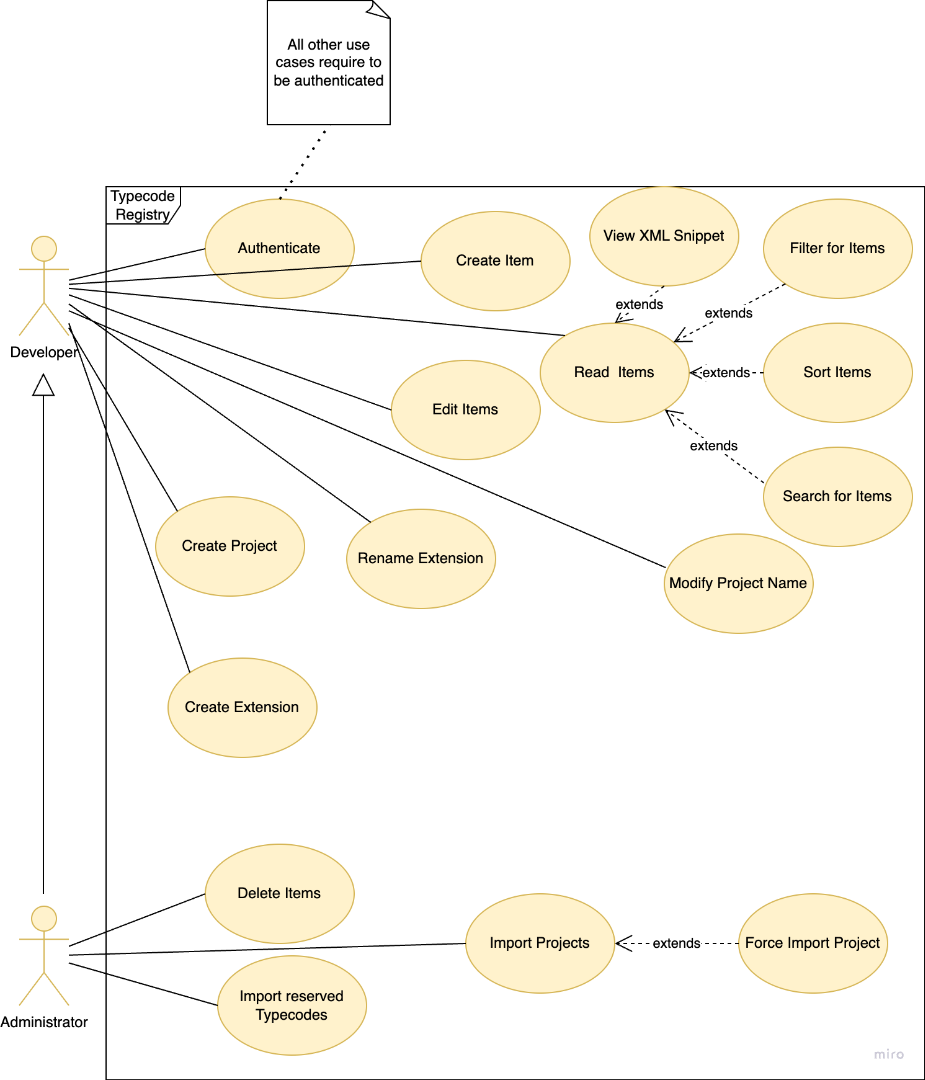
\includegraphics[scale=0.43]{images/introduction/use_cases}
\caption{Overview of the Use Cases}
\label{fig:use-cases}
\end{figure}


\subsubsection{Use Case UC-1: Create Items}\label{subsubsec:use-case-uc-1:-create-items}

\begin{table}[H]
    \centering
    \begin{tabular}{|p{0.5\textwidth}|p{0.5\textwidth}|}

        \hline
        %%% Row  Name
        \rowcolor{gray!50}\textbf{Name} & \rowcolor{gray!50}\textbf{Jira Ticket Number} \\
        UC-1 Create Items
        &
        \href{https://fh-burgenland.atlassian.net/browse/TRN-4}{TRN-4: Create Items} \\ \hline

        %% Row  User Role
        \multicolumn{2}{|l|}{\rowcolor{gray!50}\textbf{User Role}} \\
        \multicolumn{2}{|l|}{Developer} \\ \hline

        %% Row Purpse
        \multicolumn{2}{|l|}{\rowcolor{gray!50}\textbf{Purpose}} \\
        \multicolumn{2}{|l|}{Generation of an item containing a unique typecode for a project or an extension.} \\ \hline

        %% Row Preconditon & Postcondition
        \rowcolor{gray!50}\textbf{Precondition} & \rowcolor{gray!50}\textbf{Postcondition} \\
        The developer successfully logged using his Microsoft Account.
         &
        The XML Snippet of the successfully created typecode is displayed on the screen. \\ \hline

        \rowcolor{gray!50}\textbf{User Intention} & \rowcolor{gray!50}\textbf{System Response} \\
        A developer working on a project wants to create a new item needed for the project he is working on without
        the need to worry about uniqueness of the item's typecode.
         &
        The system shows a success message and the XML snippet of the created item.
        The system persisted the newly generated item in the database.
        \\ \hline

         & \\ \hline

        \multicolumn{2}{|l|}{\rowcolor{gray!50}\textbf{Remarks}} \\
        \multicolumn{2}{|p{1\textwidth}|}{Depending on the purpose of the specific item (project related/global) the typecode (value of the item) is generated in a specific range.} \\ \hline
    \end{tabular}
    \caption{UC-1: Create items}
    \label{tab:uc-1_create-items}
\end{table}

\subsubsection{Use Case UC-2: Update Items}\label{subsubsec:use-case-uc-2:-update-items}

\begin{table}[H]
    \centering
    \begin{tabular}{|p{0.5\textwidth}|p{0.5\textwidth}|}

        \hline
        %%% Row  Name
        \rowcolor{gray!50}\textbf{Name} & \rowcolor{gray!50}\textbf{Jira Ticket Number} \\
        UC-2 - Update Items
        &
        \href{https://fh-burgenland.atlassian.net/browse/TRN-33}{TRN-33: Update items} \\ \hline

        %% Row  User Role
        \multicolumn{2}{|l|}{\rowcolor{gray!50}\textbf{User Role}} \\
        \multicolumn{2}{|l|}{Developer} \\ \hline

        %% Row Purpose
        \multicolumn{2}{|l|}{\rowcolor{gray!50}\textbf{Purpose}} \\
        \multicolumn{2}{|l|}{Modify an already existing item to fit new needs.} \\ \hline

        %% Row Preconditon & Postcondition
        \rowcolor{gray!50}\textbf{Precondition} & \rowcolor{gray!50}\textbf{Postcondition} \\
        The developer successfully logged using his Microsoft Account and found the specific item he wants to modify.
        &
        The item was successfully modified and shows the edited values in the table of typecodes. \\ \hline

        \rowcolor{gray!50}\textbf{User Intention} & \rowcolor{gray!50}\textbf{System Response} \\
        A developer needs to modify an already existing item to fit new needs.
        Those could be that the item itself needs to be renamed or the table name needs to be changed.
        &
        The changes to the item are persisted in the database and the table of typecodes is updated. \\ \hline

        & \\ \hline

        \multicolumn{2}{|l|}{\rowcolor{gray!50}\textbf{Remarks}} \\
        \multicolumn{2}{|p{1\textwidth}|}{Only the name and table name of the item can be modified. When the scope, project or extension needs to be adapted, the item must be deleted and newly created } \\ \hline
    \end{tabular}
    \caption{UC-2: update items}
    \label{tab:uc-2_update items}
\end{table}

\subsubsection{Use Case UC-3: Delete items}\label{subsubsec:use-case-uc-3:-delete-items}

\begin{table}[H]
    \centering
    \begin{tabular}{|p{0.5\textwidth}|p{0.5\textwidth}|}

        \hline
        %%% Row  Name
        \rowcolor{gray!50}\textbf{Name} & \rowcolor{gray!50}\textbf{Jira Ticket Number} \\
        UC-3 - Delete items
        &
        \href{https://fh-burgenland.atlassian.net/browse/TRN-34}{TRN-34: Delete Items} \\ \hline

        %% Row  User Role
        \multicolumn{2}{|l|}{\rowcolor{gray!50}\textbf{User Role}} \\
        \multicolumn{2}{|l|}{Administrator} \\ \hline

        %% Row Purpose
        \multicolumn{2}{|l|}{\rowcolor{gray!50}\textbf{Purpose}} \\
        \multicolumn{2}{|l|}{Delete an already existing item.} \\ \hline

        %% Row Preconditon & Postcondition
        \rowcolor{gray!50}\textbf{Precondition} & \rowcolor{gray!50}\textbf{Postcondition} \\
        The developer successfully logged using his Microsoft Account and has administrator rights.
        &
        A message saying that the deletion of the item was successful is shown on the display. \\ \hline

        \rowcolor{gray!50}\textbf{User Intention} & \rowcolor{gray!50}\textbf{System Response} \\
        An administrator needs to delete an already existing item due to a conflict or other reasons.
        &
        The persisted item is the deleted from the database. \\ \hline

        & \\ \hline

        \multicolumn{2}{|l|}{\rowcolor{gray!50}\textbf{Remarks}} \\
        \multicolumn{2}{|p{1\textwidth}|}{The deletion of an item is a rare case and should be only exercised with caution.} \\ \hline
    \end{tabular}
    \caption{UC-3: Delete an item}
    \label{tab:uc-delete-an-item}
\end{table}

\subsubsection{Use Case UC-4: Read items}\label{subsubsec:use-case-uc-4:-read-items}

\begin{table}[H]
    \centering
    \begin{tabular}{|p{0.5\textwidth}|p{0.5\textwidth}|}

        \hline
        %%% Row  Name
        \rowcolor{gray!50}\textbf{Name} & \rowcolor{gray!50}\textbf{Jira Ticket Number} \\
        UC-4 - Read items
        &
        \href{https://fh-burgenland.atlassian.net/browse/TRN-35}{TRN-34: Read Items} \\ \hline

        %% Row  User Role
        \multicolumn{2}{|l|}{\rowcolor{gray!50}\textbf{User Role}} \\
        \multicolumn{2}{|l|}{Developer} \\ \hline

        %% Row Purpose
        \multicolumn{2}{|l|}{\rowcolor{gray!50}\textbf{Purpose}} \\
        \multicolumn{2}{|l|}{Read existing items from the database and display the items in a table.} \\ \hline

        %% Row Preconditon & Postcondition
        \rowcolor{gray!50}\textbf{Precondition} & \rowcolor{gray!50}\textbf{Postcondition} \\
        The developer successfully logged in using his Microsoft Account.
        &
        Existing items are listed in a table.  \\ \hline

        \rowcolor{gray!50}\textbf{User Intention} & \rowcolor{gray!50}\textbf{System Response} \\
        A developer wants to see all existing items in the system.
        &
        The items are fetched from the database and sent to the user interface displaying the items. \\ \hline

        & \\ \hline

        \multicolumn{2}{|l|}{\rowcolor{gray!50}\textbf{Remarks}} \\
        \multicolumn{2}{|p{1\textwidth}|}{None.} \\ \hline
    \end{tabular}
    \caption{UC-4: Read items}
    \label{tab:uc-read-items}
\end{table}

\subsubsection{Use Case UC-5: Display item's XML snippet.}\label{subsubsec:use-case-uc-5:-display-item's-xml-snippet}

\begin{table}[H]
    \centering
    \begin{tabular}{|p{0.5\textwidth}|p{0.5\textwidth}|}

        \hline
        %%% Row  Name
        \rowcolor{gray!50}\textbf{Name} & \rowcolor{gray!50}\textbf{Jira Ticket Number} \\
        UC-5 - Display item's XML snippet.
        &
        \href{https://fh-burgenland.atlassian.net/browse/TRN-112}{TRN-112: Display item's XML snippet} \\ \hline


        %% Row  User Role
        \multicolumn{2}{|l|}{\rowcolor{gray!50}\textbf{User Role}} \\
        \multicolumn{2}{|l|}{Developer} \\ \hline

        %% Row Purpose
        \multicolumn{2}{|l|}{\rowcolor{gray!50}\textbf{Purpose}} \\
        \multicolumn{2}{|l|}{Display Item's XML snippet to the developer.} \\ \hline

        %% Row Preconditon & Postcondition
        \rowcolor{gray!50}\textbf{Precondition} & \rowcolor{gray!50}\textbf{Postcondition} \\
        The developer successfully logged in using his Microsoft Account.
        &
        The item's XML snippet is displayed on the screen.
        The developer can use a ``Copy to clipboard`` button to copy the entire snippet to the clipboard.\\ \hline

        \rowcolor{gray!50}\textbf{User Intention} & \rowcolor{gray!50}\textbf{System Response} \\
        A developer wants to retrieve the XML snippet of a specific item to insert it to a specific project's items.xml file.
        &
        The system shows the XML snippet to the developer. \\ \hline

        & \\ \hline

        \multicolumn{2}{|l|}{\rowcolor{gray!50}\textbf{Remarks}} \\
        \multicolumn{2}{|p{1\textwidth}|}{None.} \\ \hline
    \end{tabular}
    \caption{UC-5: Display item's XML snippet.}
    \label{tab:uc-xml-snippet}
\end{table}

\subsubsection{Use Case UC-6: Filter for items.}\label{subsubsec:use-case-uc-5:-filter-for-items}

\begin{table}[H]
    \centering
    \begin{tabular}{|p{0.5\textwidth}|p{0.5\textwidth}|}

        \hline
        %%% Row  Name
        \rowcolor{gray!50}\textbf{Name} & \rowcolor{gray!50}\textbf{Jira Ticket Number} \\
        UC-6 - Filter for items.
        &
        \href{https://fh-burgenland.atlassian.net/browse/TRN-56}{TRN-56: Filter for items} \\ \hline

        %% Row  User Role
        \multicolumn{2}{|l|}{\rowcolor{gray!50}\textbf{User Role}} \\
        \multicolumn{2}{|l|}{Developer} \\ \hline

        %% Row Purpose
        \multicolumn{2}{|l|}{\rowcolor{gray!50}\textbf{Purpose}} \\
        \multicolumn{2}{|l|}{Displayed items can be filtered by name, typecode, table-name, extension and scope.} \\ \hline

        %% Row Preconditon & Postcondition
        \rowcolor{gray!50}\textbf{Precondition} & \rowcolor{gray!50}\textbf{Postcondition} \\
        The developer successfully logged in using his Microsoft Account and added the filter criteria to the filter fields.
        &
        The items table is filtered by the entered filter criteria.\\ \hline

        \rowcolor{gray!50}\textbf{User Intention} & \rowcolor{gray!50}\textbf{System Response} \\
        A developer needs to filter the viewed table by a specific filter criteria  to find a subset of items.
        &
        The table shows matching items to the filter criteria. \\ \hline

        & \\ \hline

        \multicolumn{2}{|l|}{\rowcolor{gray!50}\textbf{Remarks}} \\
        \multicolumn{2}{|p{1\textwidth}|}{None.} \\ \hline
    \end{tabular}
    \caption{UC-6: Filter for items.}
    \label{tab:uc-filter-for-items}
\end{table}

%Login & Users should be able to login by using their Microsoft Account

\subsubsection{Use Case UC-7: Sort items}\label{subsubsec:use-case-uc-7:-sort-items}

\begin{table}[H]
    \centering
    \begin{tabular}{|p{0.5\textwidth}|p{0.5\textwidth}|}

        \hline
        %%% Row  Name
        \rowcolor{gray!50}\textbf{Name} & \rowcolor{gray!50}\textbf{Jira Ticket Number} \\
        UC-7 - Sort items
        &
        \href{https://fh-burgenland.atlassian.net/browse/TRN-5}{TRN-5: Sort items} \\ \hline

        %% Row  User Role
        \multicolumn{2}{|l|}{\rowcolor{gray!50}\textbf{User Role}} \\
        \multicolumn{2}{|l|}{Developer} \\ \hline

        %% Row Purpose
        \multicolumn{2}{|l|}{\rowcolor{gray!50}\textbf{Purpose}} \\
        \multicolumn{2}{|p{1\textwidth}|}{Displayed items can be sorted by name, typecode, table-name, extension and scope.} \\ \hline

        %% Row Preconditon & Postcondition
        \rowcolor{gray!50}\textbf{Precondition} & \rowcolor{gray!50}\textbf{Postcondition} \\
        The developer successfully logged in using his Microsoft Account and clicked on the specific column he wants the item to be sorted by to sort the items.
        &
        The table displaying the items is sorted according to the specific column. \\ \hline

        \rowcolor{gray!50}\textbf{User Intention} & \rowcolor{gray!50}\textbf{System Response} \\
        A developer wants to sort the table by a specific column to order items by that context.
        &
        The table is sorted by the chosen column. \\ \hline

        & \\ \hline

        \multicolumn{2}{|l|}{\rowcolor{gray!50}\textbf{Remarks}} \\
        \multicolumn{2}{|p{1\textwidth}|}{None.} \\ \hline
    \end{tabular}
    \caption{UC-7: Sort items.}
    \label{tab:uc-sort-items}
\end{table}

\subsubsection{Use Case UC-8: Create a Project}\label{subsubsec:use-case-uc-8:-create a project}

\begin{table}[H]
    \centering
    \begin{tabular}{|p{0.5\textwidth}|p{0.5\textwidth}|}

        \hline
        %%% Row  Name
        \rowcolor{gray!50}\textbf{Name} & \rowcolor{gray!50}\textbf{Jira Ticket Number} \\
        UC-8 - Create projects
        &
        \href{https://fh-burgenland.atlassian.net/browse/TRN-89}{TRN-89: Create projects} \\ \hline

        %% Row  User Role
        \multicolumn{2}{|l|}{\rowcolor{gray!50}\textbf{User Role}} \\
        \multicolumn{2}{|l|}{Developer} \\ \hline

        %% Row Purpose
        \multicolumn{2}{|l|}{\rowcolor{gray!50}\textbf{Purpose}} \\
        \multicolumn{2}{|p{1\textwidth}|}{Create a new project by passing the name and an optional description for the project.} \\ \hline

        %% Row Preconditon & Postcondition
        \rowcolor{gray!50}\textbf{Precondition} & \rowcolor{gray!50}\textbf{Postcondition} \\
        The developer is successfully logged in using his Microsoft and selected the option on the screen for creating a new project.
        &
        The developer gets a message which confirms that the project was successfully created.\\ \hline

        \rowcolor{gray!50}\textbf{User Intention} & \rowcolor{gray!50}\textbf{System Response} \\
        A developer works on a new project and wants to reflect the project in the system.
        &
        The system approves the creation of the project. \\ \hline

        & \\ \hline

        \multicolumn{2}{|l|}{\rowcolor{gray!50}\textbf{Remarks}} \\
        \multicolumn{2}{|p{1\textwidth}|}{None.} \\ \hline
    \end{tabular}
    \caption{UC-8: Create projects.}
    \label{tab:uc-create-project}
\end{table}

\subsubsection{Use Case UC-9: Create Extensions}\label{subsubsec:use-case-uc-9:-create-extensions}

\begin{table}[H]
    \centering
    \begin{tabular}{|p{0.5\textwidth}|p{0.5\textwidth}|}

        \hline
        %%% Row  Name
        \rowcolor{gray!50}\textbf{Name} & \rowcolor{gray!50}\textbf{Jira Ticket Number} \\
        UC-9 - Create extensions.
        &
        \href{https://fh-burgenland.atlassian.net/browse/TRN-90}{TRN-90: Create extensions} \\ \hline

        %% Row  User Role
        \multicolumn{2}{|l|}{\rowcolor{gray!50}\textbf{User Role}} \\
        \multicolumn{2}{|l|}{Developer} \\ \hline

        %% Row Purpose
        \multicolumn{2}{|l|}{\rowcolor{gray!50}\textbf{Purpose}} \\
        \multicolumn{2}{|p{1\textwidth}|}{Create a new extension by passing a name and a scope to the extension. If the scope is set to project scope, then an existing project needs to be selected.} \\ \hline

        %% Row Preconditon & Postcondition
        \rowcolor{gray!50}\textbf{Precondition} & \rowcolor{gray!50}\textbf{Postcondition} \\
        The developer is successfully logged in using his Microsoft account and selected the option on the screen for creating a new project.
        &
        The developer gets a message which confirms that the extension was successfully created.\\ \hline

        \rowcolor{gray!50}\textbf{User Intention} & \rowcolor{gray!50}\textbf{System Response} \\
        A developer needs to create an extension for a project or a global extension.
        The developer selects the scope and the project if the scope is set to project scope.
        &
        The system approves the creation of the extension by showing a success message. \\ \hline

        & \\ \hline

        \multicolumn{2}{|l|}{\rowcolor{gray!50}\textbf{Remarks}} \\
        \multicolumn{2}{|p{1\textwidth}|}{None.} \\ \hline
    \end{tabular}
    \caption{UC-9: Create extensions}
    \label{tab:uc-create-extensions}
\end{table}

\subsubsection{Use Case UC-10: Rename extensions}\label{subsubsec:use-case-uc-10:-rename-extensions}

\begin{table}[H]
    \centering
    \begin{tabular}{|p{0.5\textwidth}|p{0.5\textwidth}|}

        \hline
        %%% Row  Name
        \rowcolor{gray!50}\textbf{Name} & \rowcolor{gray!50}\textbf{Jira Ticket Number} \\
        UC-10 - Rename Extensions
        &
        \href{https://fh-burgenland.atlassian.net/browse/TRN-113}{TRN-113: Rename Extensions} \\ \hline

        %% Row  User Role
        \multicolumn{2}{|l|}{\rowcolor{gray!50}\textbf{User Role}} \\
        \multicolumn{2}{|l|}{Developer} \\ \hline

        %% Row Purpose
        \multicolumn{2}{|l|}{\rowcolor{gray!50}\textbf{Purpose}} \\
        \multicolumn{2}{|p{1\textwidth}|}{Rename an already in the system existing extension.} \\ \hline

        %% Row Preconditon & Postcondition
        \rowcolor{gray!50}\textbf{Precondition} & \rowcolor{gray!50}\textbf{Postcondition} \\
        The developer is successfully logged in using his Microsoft and searched for the specific extension he wants to rename.
        &
        The table shows the extension displaying the new name.
        The new name is also persisted to the database.\\ \hline

        \rowcolor{gray!50}\textbf{User Intention} & \rowcolor{gray!50}\textbf{System Response} \\
        A developer wants to rename an already existing extension to fit new needs.
        &
        The system approves the change by showing the change in the table. \\ \hline

        & \\ \hline

        \multicolumn{2}{|l|}{\rowcolor{gray!50}\textbf{Remarks}} \\
        \multicolumn{2}{|p{1\textwidth}|}{None.} \\ \hline
    \end{tabular}
    \caption{UC-10: Rename extensions}
    \label{tab:uc-rename-extensions}
\end{table}


%F12 & Modify Project Name & A project which already exists in the system can be renamed. \\ \hline

\subsubsection{Use Case UC-11: Rename Projects}\label{subsubsec:use-case-uc-11:-rename-project}

\begin{table}[H]
    \centering
    \begin{tabular}{|p{0.5\textwidth}|p{0.5\textwidth}|}

        \hline
        %%% Row  Name
        \rowcolor{gray!50}\textbf{Name} & \rowcolor{gray!50}\textbf{Jira Ticket Number} \\
        UC-11 - Rename Projects
        &
        \href{https://fh-burgenland.atlassian.net/browse/TRN-114}{TRN-114: Rename Projects} \\ \hline

        %% Row  User Role
        \multicolumn{2}{|l|}{\rowcolor{gray!50}\textbf{User Role}} \\
        \multicolumn{2}{|l|}{Developer} \\ \hline

        %% Row Purpose
        \multicolumn{2}{|l|}{\rowcolor{gray!50}\textbf{Purpose}} \\
        \multicolumn{2}{|p{1\textwidth}|}{A project needs to be renamed due to new needs.} \\ \hline

        %% Row Preconditon & Postcondition
        \rowcolor{gray!50}\textbf{Precondition} & \rowcolor{gray!50}\textbf{Postcondition} \\
        The developer is successfully logged in using his Microsoft account.
        The developer searched for the specific project he wants to rename.
        &
        The respective project has been renamed and the change has been persisted to the database.\\ \hline

        \rowcolor{gray!50}\textbf{User Intention} & \rowcolor{gray!50}\textbf{System Response} \\
        The developer has the need to rename a project due to new needs which came up.
        &
        The project was successfully altered in the database and the new project name is displayed on the screen. \\ \hline

        & \\ \hline

        \multicolumn{2}{|l|}{\rowcolor{gray!50}\textbf{Remarks}} \\
        \multicolumn{2}{|p{1\textwidth}|}{None.} \\ \hline
    \end{tabular}
    \caption{UC-11: Rename Projects}
    \label{tab:uc-rename-projects}
\end{table}

\subsubsection{Use Case UC-12: Import reserved typecodes}\label{subsubsec:use-case-uc-12:-import-reserved-typecodes}

\begin{table}[H]
    \centering
    \begin{tabular}{|p{0.5\textwidth}|p{0.5\textwidth}|}

        \hline
        %%% Row  Name
        \rowcolor{gray!50}\textbf{Name} & \rowcolor{gray!50}\textbf{Jira Ticket Number} \\
        UC-12 - Import reserved typecodes
        &
        \href{https://fh-burgenland.atlassian.net/browse/TRN-7}{TRN-7: Import reserved typecodes} \\ \hline

        %% Row  User Role
        \multicolumn{2}{|l|}{\rowcolor{gray!50}\textbf{User Role}} \\
        \multicolumn{2}{|l|}{Administrator} \\ \hline

        %% Row Purpose
        \multicolumn{2}{|l|}{\rowcolor{gray!50}\textbf{Purpose}} \\
        \multicolumn{2}{|p{1\textwidth}|}{Administrators can import internal system typecodes via a ``reservedTypecodes.txt`` file} \\ \hline

        %% Row Preconditon & Postcondition
        \rowcolor{gray!50}\textbf{Precondition} & \rowcolor{gray!50}\textbf{Postcondition} \\
        The administrator has a txt file containing proper reserved typecodes.
        &
        Reserved typecodes have been imported successfully.\\ \hline

        \rowcolor{gray!50}\textbf{User Intention} & \rowcolor{gray!50}\textbf{System Response} \\
        The administrator wants to import reserved typecodes via a ``reservedTypecodes.txt`` file.
        &
        The client sends a POST request to the server and the projects are imported. \\ \hline

        & \\ \hline

        \multicolumn{2}{|l|}{\rowcolor{gray!50}\textbf{Remarks}} \\
        \multicolumn{2}{|p{1\textwidth}|}{None.} \\ \hline
    \end{tabular}
    \caption{UC-12: Import reserved typecodes}
    \label{tab:uc-import-reserved-typecodes}
\end{table}

\subsubsection{Use Case UC-13: Import projects via XML files}\label{subsubsec:use-case-uc-13:-import-projects-via-xml-files}

\begin{table}[H]
    \centering
    \begin{tabular}{|p{0.5\textwidth}|p{0.5\textwidth}|}

        \hline
        %%% Row  Name
        \rowcolor{gray!50}\textbf{Name} & \rowcolor{gray!50}\textbf{Jira Ticket Number} \\
        UC-13 - Import Projects via XML files
        &
        \href{https://fh-burgenland.atlassian.net/browse/TRN-115}{TRN-115: Import projects via XML files} \\ \hline

        %% Row  User Role
        \multicolumn{2}{|l|}{\rowcolor{gray!50}\textbf{User Role}} \\
        \multicolumn{2}{|l|}{Administrator} \\ \hline

        %% Row Purpose
        \multicolumn{2}{|l|}{\rowcolor{gray!50}\textbf{Purpose}} \\
        \multicolumn{2}{|l|}{Administrators can import new projects via XML files.} \\ \hline

        %% Row Preconditon & Postcondition
        \rowcolor{gray!50}\textbf{Precondition} & \rowcolor{gray!50}\textbf{Postcondition} \\
        The administrator has an XML file containing proper project items.
        &
        Projects have been imported successfully.\\ \hline

        \rowcolor{gray!50}\textbf{User Intention} & \rowcolor{gray!50}\textbf{System Response} \\
        An administrator wants to import new projects via an XML file.
        &
        The client sends a POST request to the server and the projects are imported. \\ \hline

        & \\ \hline

        \multicolumn{2}{|l|}{\rowcolor{gray!50}\textbf{Remarks}} \\
        \multicolumn{2}{|p{1\textwidth}|}{The systems allows duplicates but marks them as conflicts once they have been imported.} \\ \hline
    \end{tabular}
    \caption{UC-13: Import projects via XML files}
    \label{tab:uc-import-projects-via-xml-files}
\end{table}

\subsubsection{Use Case UC-14: Login via microsoft account}\label{subsubsec:use-case-uc-14:-login-via-microsoft-account}

\begin{table}[H]
    \centering
    \begin{tabular}{|p{0.5\textwidth}|p{0.5\textwidth}|}

        \hline
        %%% Row  Name
        \rowcolor{gray!50}\textbf{Name} & \rowcolor{gray!50}\textbf{Jira Ticket Number} \\
        UC-14 - Login via Microsoft account.
        &
        \href{https://fh-burgenland.atlassian.net/browse/TRN-2}{TRN-2: Login via Microsoft Account} \\ \hline

        %% Row  User Role
        \multicolumn{2}{|l|}{\rowcolor{gray!50}\textbf{User Role}} \\
        \multicolumn{2}{|l|}{Developer} \\ \hline

        %% Row Purpose
        \multicolumn{2}{|l|}{\rowcolor{gray!50}\textbf{Purpose}} \\
        \multicolumn{2}{|l|}{Users can log into the registry via their microsoft account.} \\ \hline

        %% Row Preconditon & Postcondition
        \rowcolor{gray!50}\textbf{Precondition} & \rowcolor{gray!50}\textbf{Postcondition} \\
        The developer is shown the login mask and has entered their login data correctly.
        &
        The user has been logged in and is shown the dashboard.  \\ \hline

        \rowcolor{gray!50}\textbf{User Intention} & \rowcolor{gray!50}\textbf{System Response} \\
        A developer wants to log into the registry.
        &
        The system authenticates and grants access to the developer. \\ \hline

        & \\ \hline

        \multicolumn{2}{|l|}{\rowcolor{gray!50}\textbf{Remarks}} \\
        \multicolumn{2}{|p{1\textwidth}|}{Microsoft Entra shall be used for identification.} \\ \hline
    \end{tabular}
    \caption{UC-14: Login via microsoft account}
    \label{tab:uc-login-via-microsoft-account}
\end{table}

\subsubsection{Use Case UC-15: Logout from Typecode-Registry}\label{subsubsec:use-case-uc-15:-logout}

\begin{table}[H]
    \centering
    \begin{tabular}{|p{0.5\textwidth}|p{0.5\textwidth}|}

        \hline
        %%% Row  Name
        \rowcolor{gray!50}\textbf{Name} & \rowcolor{gray!50}\textbf{Jira Ticket Number} \\
        UC-15 - Logout from Typecode-Registry
        &
        \href{https://fh-burgenland.atlassian.net/browse/TRN-116}{TRN-116: Logout from Typecode-Registry} \\ \hline

        %% Row  User Role
        \multicolumn{2}{|l|}{\rowcolor{gray!50}\textbf{User Role}} \\
        \multicolumn{2}{|l|}{Developer} \\ \hline

        %% Row Purpose
        \multicolumn{2}{|l|}{\rowcolor{gray!50}\textbf{Purpose}} \\
        \multicolumn{2}{|l|}{Allow the user to log out.} \\ \hline

        %% Row Preconditon & Postcondition
        \rowcolor{gray!50}\textbf{Precondition} & \rowcolor{gray!50}\textbf{Postcondition} \\
        The developer successfully logged in using his Microsoft account.
        &
        The user has been logged out and is shown the login mask.  \\ \hline

        \rowcolor{gray!50}\textbf{User Intention} & \rowcolor{gray!50}\textbf{System Response} \\
        A developer wants to log out from the registry.
        &
        The system logs the user out. \\ \hline

        & \\ \hline

        \multicolumn{2}{|l|}{\rowcolor{gray!50}\textbf{Remarks}} \\
        \multicolumn{2}{|p{1\textwidth}|}{None.} \\ \hline
    \end{tabular}
    \caption{UC-15: Logout}
    \label{tab:uc-logout}
\end{table}

\subsection{Technology Stack}

In the construction of our application, careful consideration was given to the selection of the technology stack to ensure optimal performance, maintainability, and alignment with the client's existing technological ecosystem.

\begin{itemize}
    \item \textbf{Backend:} Golang was chosen for the backend development due to its performance efficiency and simplicity.
    Go's straightforward syntax and powerful standard library enable rapid development and maintenance.
    While Java Spring Boot is a robust alternative, Golang's lightweight nature and concurrency model provide superior performance for containerized microservices.
    Moreover, Golang aligns with the client's technology stack, allowing for better integration and utilization of in-house expertise.

    \item \textbf{Frontend:} Angular is our choice for the frontend framework due to its comprehensive solution for developing scalable single-page applications.
    It offers a robust structure for managing complex components and their lifecycle, which is crucial for the long-term maintainability of the frontend codebase.

    \item \textbf{Database:} PostgreSQL was selected as the database for its advanced features, reliability, and strong community support.
    It provides the necessary scalability and data integrity guarantees required for the application.

    \item \textbf{Deployment:} Docker and Kubernetes are utilized for deployment, offering a containerized environment that ensures consistency across development, testing, and production.
    Kubernetes adds a layer of orchestration for Docker containers, enhancing the application's availability and scalability.
\end{itemize}

The technology choices reflect a commitment to modern, reliable, and efficient software development practices, ensuring that the application is both high-performing and sustainable over time.

